%&LaTeX

\section{Feedforward Filters}

This lab covers the basic concepts of filtering and feedforward filters. 
You may have also heard of feedforward filters referred to as 
finite impulse response (FIR) filters. In this lab, we will cover the basic idea
of a filter, its mathematical representation (such as the defining equation,
frequency response, and transfer function), the relationship among
filter coefficients, zero placement, and filter type (low pass, high
pass, band reject), and some basic properties of filters.


\subsection{Overview of Filtering and J-DSP}

A \emph{digital filter} is a signal processing operation that can be
  described equivalently by its \emph{defining
  equation}, \emph{transfer function}, or \emph{frequency response}. 
  Each representation completely defines the filter. It is advantageous 
  to use each of the different representations depending on whether you are
  \emph{implementing}, \emph{analyzing}, or \emph{designing} an FIR filter:
\begin{eqnarray*}
  y[n] &=& \underbrace{\sum_{k=0}^M b_k x[n-k]}_{\text{defining equation}} \\ 
  \hline \\
  Y &=& H(z) X\\
  H(z) &=& \underbrace{\sum_{k=0}^M b_k z^{-k}}_{ \text{transfer function} } \\
  \hline \\
  Y &=&  \mathcal{H}({\hat{\omega}}) X \\
  H(e^{j\hat{\omega}})  = \mathcal{H}({\hat{\omega}}) 
  &=& \underbrace{\sum_{k=0}^M b_k e^{-j \hat{\omega}k}}_{\text{frequency response}} 
\end{eqnarray*}

In these equations, $x[n]$ and $y[n]$ are the $n^\mathrm{th}$ samples
from the input and output, respectively, while $X$ and $Y$ represent
the entire input and output signal (all of the samples in the
signal). A $k$-sample time delay of a signal is produced by
multiplication by the delay operator, $z^{-1} = e^{-j
  \hat{\omega}k}$. In all three cases (but most simply for the
transfer function), we can obtain insight into the filter's operation
from the \emph{coefficients}, $b_k$. We can do this by factoring the
transfer function polynomial: its roots are the \emph{zeros} of the
filter and they can be real or complex.  The placement of the zeros in
the complex plane (most usefully expressed in polar coordinates) will
tell us which frequencies are suppressed and to what extent those
frequencies are suppressed (we can calculate each using the angle and
magnitude of the zero, respectively).

\begin{figure}
  \begin{center}
    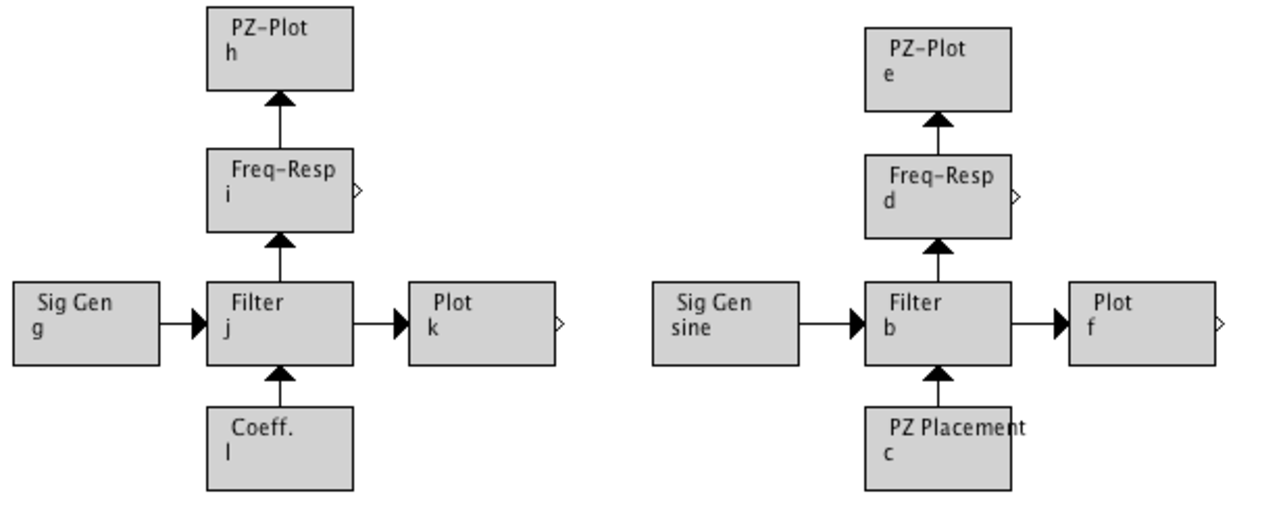
\includegraphics[width=5in]{lab4/polezerodiagrams}
  \end{center}
  \caption{J-DSP setup for specifying filter coefficients and monitoring
  frequency response and zero location. (Left) Using the \block{coeff} block. (Right) Using the \block{PZ-Placement} block
  \label{fg:PZfigs}}
\end{figure}

J-DSP has a set of blocks that directly correspond to the concepts we
have learned. These include the \block{Filter} block, which takes an
input signal on the left and parameters (zero locations or
coefficients) at the bottom, and produces an output signal on the
right and can have its characteristics (frequency response or zero
locations) monitored via a connection from the top. We will use
\block{Filter} in two different ways:
\begin{enumerate}
\item We will specify the coefficients of the transfer function or
  generating equation using the \block{Coeff.} block and monitor the
  filter's output (using \block{Plot}), frequency response (using
  \block{Freq-Resp}), and zero placement (using \block{PZ-Plot}), as
  in Figure~\ref{fg:PZfigs} (left).
\item Instead of defining the filter using the \block{Coeff} block, we will
  place zeros directly in the complex plane using the \block{PZ
    Placement} block (which has an option to show the corresponding
  filter coefficients), as shown in Figure~\ref{fg:PZfigs} (right).
\end{enumerate}
Remember, we can define a specific filter using either of the methods
above. Sometimes it is easier to understand the filter using zeros and
sometimes it is easier to use the coefficients directly.  Either
method can be used to represent the same filter.


\subsubsection{From Filter Coefficients to Transfer Function and Frequency Response}

Given the coefficients of an FIR filter we can solve for the zero
locations and the frequency response.  For example the two-point
averaging system is given by:
\[
y[n] = \frac{1}{2}x[n] + \frac{1}{2}x[n-1]
\]
we can find the transfer function by rewriting the filter using the
delay operator, $z$:
\begin{eqnarray}
  Y    & = & \frac{1}{2} X + \frac{1}{2} z^{-1} X \\
  H(z) & = & \frac{Y}{X} = \frac{1}{2} (1 +  z^{-1})
\end{eqnarray}
If we're interested in the \emph{zero location} we can then multiply
$H(z)$ by $z/z$ to obtain:
\begin{equation}
  H(z) = \frac{\frac{1}{2} (z + 1)}{z}
\end{equation}
The root of the numerator, $z=-1$ is the location of the only zero
(the root(s) of the denominator for an FIR filter are always at $z=0$,
and do not affect the frequency response). We can also derive the frequency response from this by remembering that 
$H(e^{j\hat{\omega}})  = \mathcal{H}({\hat{\omega}})$ or that $z=e^{j\hat{\omega}}$. From the zero
location, $z=-1$, we can immediately tell that the frequency response is zero at $e^{j\hat{\omega}}=-1$ or 
$\hat{\omega}=\pi$. With a zero at an angle of
$\hat{\omega}=\pi$, this is a low-pass filter. As a warm-up, use the
J-DSP setup of Figure~\ref{fg:PZfigs} (left) to verify the expected zero
placement and frequency response.

\subsubsection{From Zero Placement to Filter Coefficients}

When we are given the zero placement, we can very easily determine the
filter coefficients because those zeros are the roots of a factored
polynomial. For example, given two complex conjugate zeros, $z_1$ and
$z_2$ (i.e., the real parts are equal, $\Real[z_{1}] = \Real[z_{2}] =
\Real[z_{1,2}] $, and the imaginary parts are negatives of one another
$ \Imag[z_{1}] = -\Imag[z_{2}] $ or, equivalently in polar
coordinates, $z_{1} = r e^{j\hat{\omega_0}}$ and $z_{2} = r
e^{-j\hat{\omega_0}}$), the transfer function is:
\begin{eqnarray}
  H(z) & = & (z - z_1)(z - z_2)/z^2 \\
  & = & (z^2 - (z_1 + z_2) z + z_1 z_2)/z^2 \\
  & = & 1 - 2 \Real[{z_{1,2}}] z^{-1} + r^2 z^{-2} \\
  & = & 1 - 2 \Real[r(\cos(\omega_0) \pm j\sin(\omega_0))] z^{-1} + r^2 z^{-2} \\
  & = & \underbrace{1}_{b_0} -\underbrace{2 r\cos(\omega_0)}_{b_1} z^{-1} + \underbrace{r^2}_{b_2} z^{-2}
\end{eqnarray}
At this point, we can rewrite the transfer function as the filter's
generating equation, using the delay operator $z^{-k}$, $y[n] = x[n] -
2 r\cos(\omega_0)x[n-1] + r^2 x[n-2]$. This allows us to read off the
filter coefficients: $b_0 = 1$, $b_1 = -2 r\cos(\omega_0)$, and $b_2 =
r^2$.

\subsection{Frequency Response and Pole-Zero Plots}

\paragraph{Step 1.1} Consider a filter that computes a running average
of three points of our input signal (a \emph{three-point averager}):
\begin{equation}
y[n] = \frac{1}{3} \sum_{k=0}^2 x[n-k] 
     = \frac{1}{3}x[n] + \frac{1}{3}x[n-1] + \frac{1}{3}x[n-2]
\end{equation}

\begin{enumerate}\renewcommand{\theenumi}{\alph{enumi}}
\item Draw a block diagram for this filter.


\item How many zeros will this filter have?


\item Find and sketch the zero locations using pencil and paper, then
  use J-DSP to verify this.

\item Sketch the magnitude of the frequency response as a function of
	$\hat{\omega}$ from the plot of pole locations and verify this using
	J-DSP. How does the minimum of the magnitude of the frequency
	response relate to the polar representation of the zero locations?
	What kind of filter would you say this is?

\end{enumerate}

\begin{figure}
  \begin{center}
    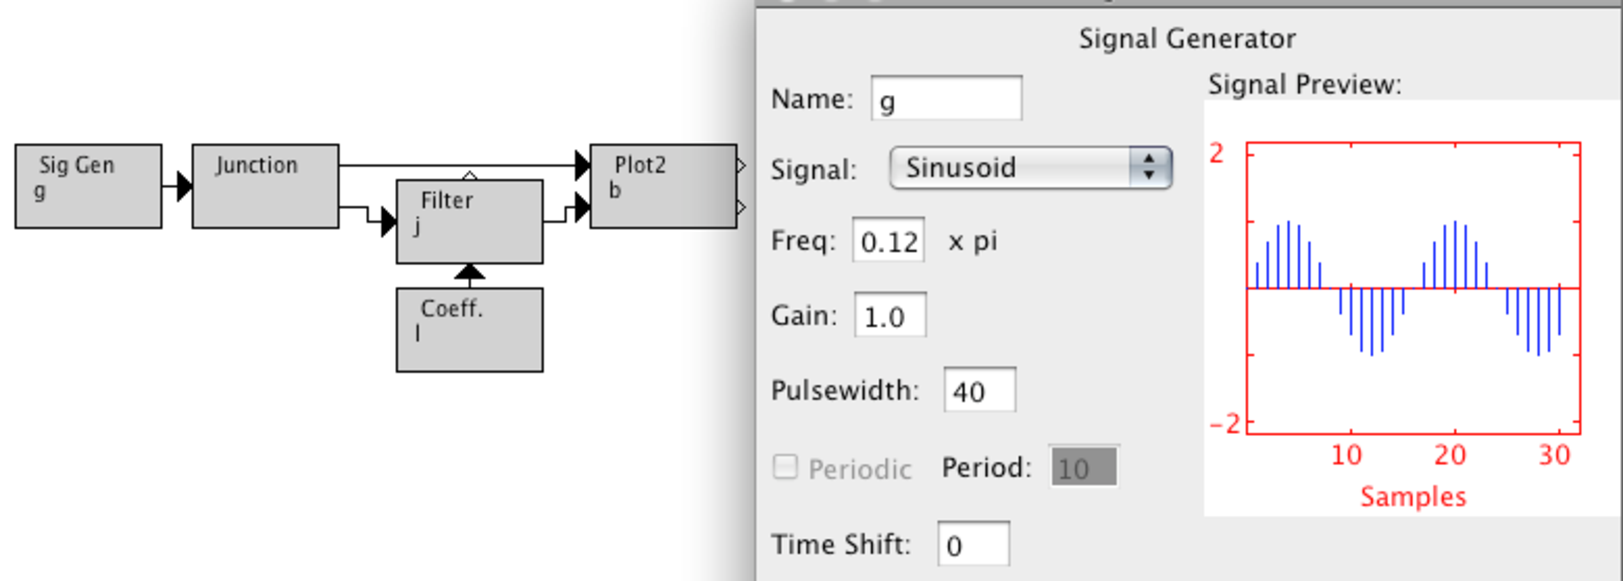
\includegraphics[width=6in]{lab4/filteredsignal}
  \end{center}
\caption{J-DSP setup for Step 1.2 (e, f, and g). \label{fg:filtsig}}
\end{figure}

\paragraph{Step 1.2} A \emph{first-difference} filter is an
approximation to a discrete derivative operation. Its defining
equation is:
\begin{equation}
  y[n] = x[n] - x[n-1]
\end{equation}

\begin{enumerate}\renewcommand{\theenumi}{\alph{enumi}}

\item Draw a block diagram for this filter.


\item Derive the transfer function, $H(z)$, for this filter. From
	  this, determine the expression for the frequency response,
	  $\mathcal{H}(\hat{\omega})=H(e^{j\hat{\omega}})$.


\item From the transfer function, determine the filter's zero
	locations and sketch them. Check your results with J-DSP.


\item From the zero plot, sketch the magnitude of the filter's
	  frequency response as a function of $\hat{\omega}$. Use J-DSP to
	  check your results. What kind of filter would you say this is?
	  

\item Use J-DSP to simulate this filter's response to the following
	  input. Set the \block{Sig Gen} to produce a sinusoid with
	  \option{frequency} $0.125\pi$, \option{gain} 1, \option{pulsewidth}
	  40. The diagram is shown in Figure \ref{fg:filtsig}.

\item Examine the plots of $X$ and $Y$ in J-DSP. Note that $Y$ appears
	  to be a scaled and shifted sinusoid of the same frequency as
	  $X$. The exception is the first point, $y[0]$. Explain why $y[0]$ is
	  different.


\item Estimate the frequency, amplitude, and phase of $Y$ directly
	  from its plot (ignoring $y[0]$).


\item To compare these measurements to theory, use your expression for
	  the filter's frequency response to calculate the amplitude and phase
	  at a frequency of $\hat{\omega} = \pi/8$. How do these compare to
	  what you determined from the J-DSP plots?


\end{enumerate}

\paragraph{Step 1.3} Just as we can compute a discrete first
derivative with a first-difference filter, we can compute a discrete
second derivative with a \emph{second difference filter}.

\begin{enumerate}\renewcommand{\theenumi}{\alph{enumi}}
\item Use your expression for the transfer function of the first
	  difference filter and your knowledge that the combined transfer
	  function of two filters cascaded, or connected in series, is the
	  product of their individual transfer functions to determine the
	  transfer function for a second-difference filter.


\item Draw a block diagram for this filter.
	

\item Determine the filter's zero locations and sketch them. Check
	  your results using J-DSP.
	  
	  

\item From the zero plot, sketch the magnitude of the filter's
	  frequency response as a function of $\hat{\omega}$. Use J-DSP to
	  check your results. What kind of filter would you say this is?


\end{enumerate}


\paragraph{Step 1.4} Consider a feedforward filter with complex
conjugate zeros at $z_{1,2} = -0.5 \pm j 0.5$.

\begin{enumerate}\renewcommand{\theenumi}{\alph{enumi}}
\item Determine the filter coefficients.


\item Use J-DSP to plot the frequency response of the filter.

\item What are the effects of the zeros on the frequency response?
	  What kind of filter would you call this?

\end{enumerate}

\subsection{Linearity and Cascading Filters}

\paragraph{Step 2.1} A system is called \emph{linear} if a sum of
different inputs produces an output that is the sum of the outputs for
the inputs taken individually.  Perform a simple test of the linearity
of this filter by doubling the input amplitude in J-DSP ($X' = 2X = X
+ X$). How does the new output amplitude compare to the old one?


\paragraph{Step 2.2} In one of the self-test exercises in the class notes,
	two filters with transfer functions $H_1(z) = b_0 + b_1z^{-1}$ and
	$H_2(z) = b'_0 + b'_1z^{-1}$ were connected in series, and it was
	shown that they could be connected in either order to produce the same
	composite effect (the same overall transfer function). Redo this
	exercise using the \emph{defining equations} for the two filters, i.e.,
	$y_1[n] = F_1(x[n])$ for the filter with transfer function $H_1(z)$
	and $y_2[n] = F_2(x[n])$ for the filter with transfer function
	$H_2(z)$. In other words, show that $F_2(F_1(x[n])) =
	F_1(F_2(x[n]))$.


\paragraph{Step 2.3} Use J-DSP to implement a system in which the output of
	the \block{Sig Gen} is connected to the three-point averager of step
	1.1, the output of which is in turn connected to the first-difference
	filter of step 1.2. Set the \block{Sig Gen} to output a periodic,
	rectangular waveform with amplitude of 1, pulse width of 10, and
	period of 20. This is a 50\% duty cycle square wave. Plot the final
	output waveform. What does it look like?


\paragraph{Step 2.4} Change your J-DSP simulation so that the first
	difference filter is first and the three-point averager is
	second. Plot the output. How does the output of this configuration
	compare to that of step 3.3?


% LocalWords:  WebQ MATLAB
